
\section{Road Generation}\label{sec:road-generation}

\renewcommand{\kapitelautor}{Autor: Felix Zwickelstorfer}

Die Generierung von Straßen ist ein sehr wichtiger Punkt in Forty-Five, da es bei einem neuen Durchlauf für Abwechslung für den Spieler sorgt.
Es gibt bei der Erstellung von Roads bestimmte Parameter, damit trotzdem noch bestimmte Randbedingungen erfüllen wie beispielsweise, dass immer die gleichen Texturen als Dekorationen verwendet werden.
Im Folgenden wird nun die Entstehung einer Straße und die dabei gesetzten Parameter näher gebracht.

\subsection{Node Generation}\label{subsec:node-generation}
Um eine Straße zu generieren, braucht man als erstes Nodes, also Punkte in einem Koordinatensystem.
Diese werden wiederum anhand von sogenannten \inlineCode{MapNodeLine} erstellt und anschließend miteinander verbunden.

\subsubsection{Line Generation}\label{subsubsec:line-generation}
Eine Linie nimmt mehrere Parameter: die Anzahl der nodes, die Abstände dazwischen, und die maximale Breite, welche eine Linie zur Verfügung hat.
Linien werden immer in Richtung rechts gebaut, und erst am Ende wird die gesamte Road rotiert.
Die erste Linie, die generiert wird, funktioniert etwas anders als die anderen, da diese weniger Einschränkungen hat.
Dies geschieht folgendermaßen:

\begin{enumerate}
    \item Die Hauptlinie wird als erstes erstellt und beginnt mit dem Punkt~(0|0).
    \item Es werden \inlineCode{nbrOfPoints} weitere Punkte generiert, wobei folgende Kriterien gelten, die alle als Einschränkungen der Map angegeben werden:
    \begin{itemize}
        \item Er hat einen Mindest- und Maximalabstand in sowohl x als auch y Richtung vom vorherigen Punkt.
        \item Er hat einen maximalen Winkel vom vorherigen Punkt.
        \item Er kann hat einen maximalen Breitenabstand zu dem ersten Punkt auf der Linie.
    \end{itemize}
    \item Anschließend wird eine zufällige Richtung ausgewählt, in der die nächste Linie generiert wird, entweder darüber oder darunter.
    Diese ist immer um genau einen Punkt kürzer als die davor.
    Das stellt sicher, dass keine Linie länger sein kann als die Hauptlinie, und dass es im Normalfall auch nicht zu stark am Ende abschneidet.
    \item Der neue Startpunkt ist die Hälfe eines normalen Punktes in x-Richtung und dann um die maximal erlaubte Breite in y-Richtung nach oben oder unten, je nachdem was davor entschieden wurde.
    \item Anschließend werden wieder gleich die Nodes berechnet wie bei der Hauptlinie, nur dass ein zusätzlicher Punkt dazukommt:
    Der Abstand zu der davorliegenden Linie darf in einem Bereich um den zu planierenden Punkt nicht zu weit entfernt sein.
    Dies vermeidet, dass die Abstände zwischen zwei Linien nicht zu groß sind und dadurch auseinandergehen.
    Dies wird an der darauffolgenden Grafik~\ref{fig:point-generation} deutlich gezeigt.
    \item Dann werden Punkt drei bis fünf so oft wiederholt, wie \inlineCode{maxLines} angibt.
\end{enumerate}

\begin{figure}[H]
    \centering
    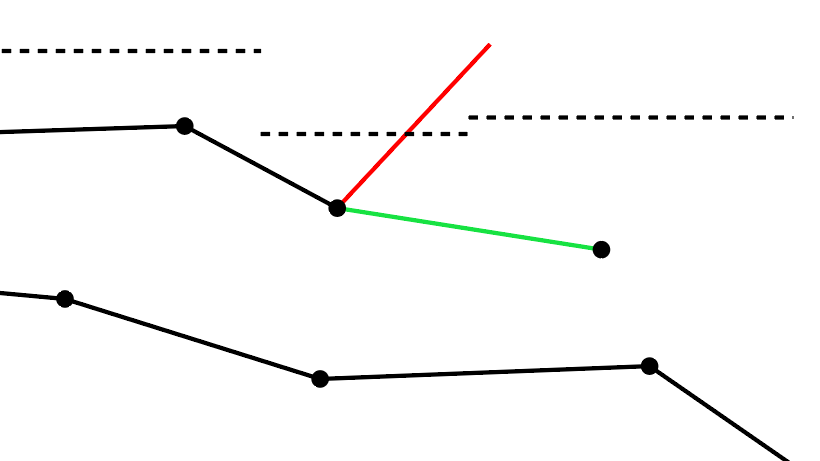
\includegraphics[width=0.7\textwidth]{node_generation_example.png}
    \caption{Beispiel: Punktegenerierung mit fehlerhafter Platzierung}\label{fig:point-generation}
\end{figure}
Die Grafik zeigt, wie bei der Generierung der Punkt am Ende der roten Linie überprüft wird, ob er platziert werden kann.
Dabei überschreitet sie allerdings den maximalen Abstand zu den darunter liegenden Linien, welcher durch die strichlierten Linien dargestellt wird.
Dadurch wird der Punkt gelöscht und ein Neuer wird generiert.
Falls dies dreimal hintereinander nicht funktioniert, wird die x-Koordinate des letzten Punktes übernommen und für die y-Koordinate wird ein zufälliger Wert im erlaubten Bereich genommen.


\subsubsection{Node Verbindungen}\label{subsubsec:node-verbindungen}
Nachdem nun eine Sammlung an Nodes vorhanden ist, werden diese miteinander Verbunden.
Dabei bekommt jedes Node einen freien Platz für jede Richtung, damit nicht zu viele Nodes in die gleiche Richtung miteinander verbunden werden.
Außerdem wird dadurch die maximale Anzahl an Verbindungen pro Node auf vier limitiert.
Dies ist wichtig, da man mit jeder Pfeiltaste in nur eine Richtung gehen kann und trotzdem jedes Feld erreichbar sein soll.
Anschließend wird die Hauptlinie komplett verbunden, wodurch ein Weg zum Ende der Straße sichergestellt wird.
Daraufhin wird bei jedem dieser Nodes eine Zufallszahl generiert und falls diese einen gewisseen Wert überschreitet, wird eine neue Verbindung in eine zufällige Richtung gestartet.
Diese Verbindung geht nach folgenden Schritten:
\begin{enumerate}
    \item Es wird die Anzahl der gewünschten Verbindeungen zu neuen Nodes mit folgender Formel berechnet: \[ \sqrt{rndValue * maxValue * 3 + 0.8}\]
        Dabei ist \inlineCode{rndValue} eine zufällige Zahl, welche mittels dem Seed generiert wird und maxValue die Anzahl der offenen Verbindungsfelder.
    \item Anschließend werden Nodes gesucht, welche Verbindungen ermöglichen.
    Diese müssen folgende Kriterien erfüllen:
    \begin{itemize}
        \item Es kann entweder das nächste auf der aktuellen Linie, oder eines der nächsten drei Punkte auf der darüber- oder darunterliegenden Linie sein.
        \item Es darf keine Verbindung in die Richtung des Ausgangspunktes geben.
        Dabei gibt es allerdings immer zwei mögliche Verbindungen, da es \zB wenn es eine Verbindung circa im 45 Grad Winkel versucht, sowohl der linke aus auch untere Slot infrage kommen.
    \end{itemize}
    \item Anschließend werden, falls vorhanden, zufällige von den möglichen Nodes ausgewählt und eine Verbindung dorthin erstellt.
    \item Diese Prozess wird so oft wiederholt, bis entweder die gewünschte Anzahl der Verbindungen null ist, oder die Hauptlinie wieder erreicht.
    Das Beenden beim Erreichen der Hauptlinie sorgt dafür, dass der Verlauf der Straße sich langsam öffnet und wieder schließt.
    Würde man dies nicht machen, gäbe es einerseits zu viele Verbindungen, und andererseits sind am Ende zu viele "lose" übrig, die weg vom eigentlichen Ziel zeigen.
\end{enumerate}

\subsubsection{Verbindungen löschen}\label{subsubsec:verbindungen-loeschen}
Da die Linien nach dem Verbinden stark durcheinander sein könnten, werden sie bevor sie fertig sind, noch überprüft.
Wenn beispielsweise zwei Linien einander überschneiden, wird versucht, ein neuer Punkt dazwischen zu platzieren, damit es zu keinen Überschneidungen kommt.
Weiteres wird eine Linie gelöscht, wenn mindestens einer der nach folgenden Punkte erfüllt ist:
\begin{itemize}
    \item Zwei Linien überschneiden einander.
    Dabei muss der Überschneidungspunkt sehr nahe an einem der Punkte sein.
    Dies wird mit dem Parameter \inlineCode{pathTotalWidth} festgelegt.
    \item Die Verlängerung einer Linie geht in eine andere Linie hinein.
    Dies weird bei der darauffolgenden Abbildung~\ref{fig:line-deletion} weiter erklärt.
    \item Zwei Nodes sind zu nah zueinander.
    Dabei wird nicht nur eine Linie, sondern ein ganzes Node gelöscht.
\end{itemize}

Im Folgenden wird gezeigt, wie die verlängerte Linie von zwei Nodes mit einer gewöhnlichen Verbindung überschneidet und dadurch auch der Löschprozess eingeleitet wird.
\begin{figure}[H]
    \centering
    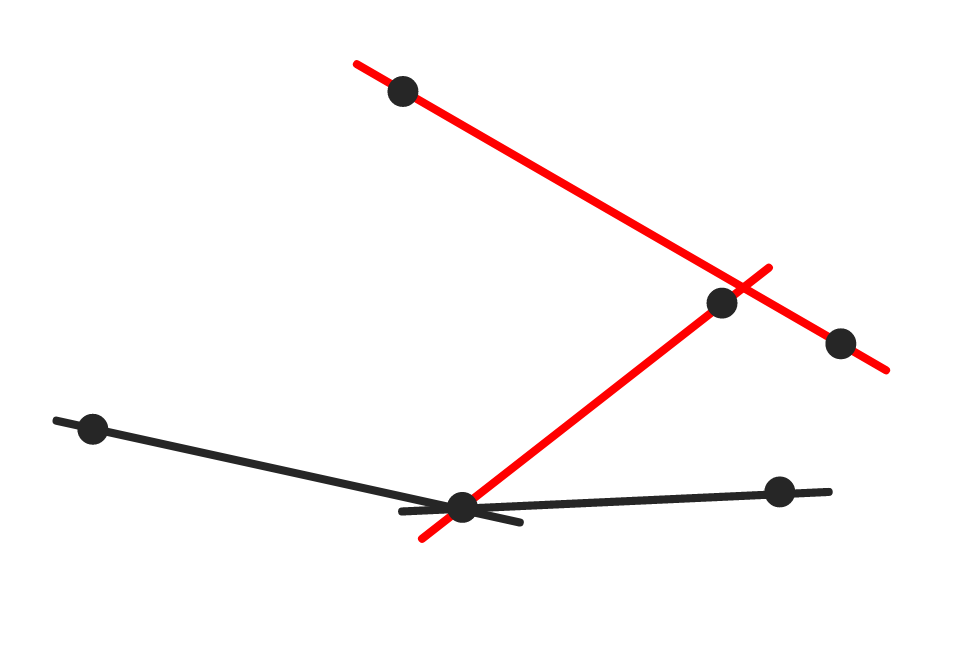
\includegraphics[width=0.7\textwidth]{line_deletion_example.png}
    \caption{Beispiel: Punktegenerierung mit fehlerhafter Platzierung}\label{fig:line-deletion}
\end{figure}

Beim Löschen von Linien geht das Programm folgendermaßen vor:
\begin{enumerate}
    \item Wenn eines der beiden Linien als Eckpunkt mindestens ein Node auf der Hauptlinie hat, wird die andere gelöscht.
    \item Wenn eine Linie ein anderes Node zu nahe überschneidet, wird diese gelöscht, da es besser ist, nur eine Linie anstatt ein ganzes Node zu löschen.
    \item Ansonsten wird zufällig entschieden, welche Linie wegkommt.
\end{enumerate}

Wenn ein Node gelöscht werden muss, wird wieder überprüft, ob eines der beiden auf der Hauptlinie ist und sollte dies der Fall sein, wird das andere gelöscht.
Durch die Art und Weise wie die Hauptlinie generiert wird, kann es niemals sein, dass sich zwei Hauptlinien überscheiden oder dass zwei Nodes einander zu nahe sind.
Falls beim Überprüfen, ob alle Linien correct und erlaubt sind, ein Fehler auftritt und etwas geändert werden muss, wird es nochmals wiederholt.
Das liegt daran, da beispielsweise ein hinzugefügtes Node oder dessen Linien mit Anderen wieder überschneiden könnten.

\subsubsection{Areas}\label{subsubsec:ares}
Areas sind statisch definiert und jede Road hat immer eine am Anfang und Ende.
Es gibt allerdings auch noch die Möglichkeit, innerhalb einer Straße weitere Areas zu haben.
Diese werden an einem der verbundenen Randpunkte zufällig mit einer verstärkten Distanz hinzugefügt, damit diese deutlich erkennbar sind.
Es erlaubt bei Erweiterungen der Storyline in der Zukunft, dass beispielsweise ein Versteck auf einer Straße zu finden ist.


\subsection{Events}\label{subsec:events}
Nachdem alle Nodes verbunden sind brauchen diese noch Events, die der Spieler ausführen kann.
Ein Node kann immer nur ein Event beinhalten.
Allerdings ist es möglich, dass auf dieses direkt ein Folgeevent auftritt, wie \zB nach einem Kampf kann man manchmal eine neue Karte bekommen.
In Onj kann jedes Event einem von drei Arten angehören:

\begin{enumerate}
    \item Fixed Events: Sind Events, die immer genau einmal vorkommen.
    Diese haben noch die Zusatzoption, dass sie, falls möglich, an eine Sackgasse kommen, also an ein Node mit nur einer Verbindung.
    Man kann auch mehrmals ein Event vom selben Typen hinzufügen, falls man es öfter haben möchte.
    \item Optional Events: Diese kommen dran, wenn noch Nodes frei sind nach den fixen Events.
    Diese haben auch eine Gewichtung, damit manche Events wie Kämpfe öfter vorkommen als \zB ein Heilevent.
    \item Final Event: Das finale Event ist immer das letzte Element auf einer Road und ist dadurch Pflicht für den Spieler.
    Dieses Event ist allerdings optional und wir meistens für einen Endboss verwendet.
    Es ist unabhängig von dem wirklich letzten Element, mit dem man die Road wieder verlässt.
\end{enumerate}

Es gibt verschiedenste Events in Forty-Five wie den Kampf, das Wechseln zwischen Road und Area, diverse Heilmöglichkeiten als auch den Shop.
Die letzten beiden werden im Folgenden erklärt.

\subsubsection{Shop}\label{subsubsec:shop}
Im Shop kann der Spieler mit dem gewonnenen Geld Karten kaufen.
Die Auswahl an Karten wird anhand eines Seeds festgelegt.
Dieser wird beim ersten Öffnen des Shops generiert.
Dadurch, dass alles von einem Seed abhängig ist, werden nicht die einzelnen Karten gespeichert, sondern nur der index der Gekauften.
Weiteres kann der Spieler beim Kauf auswählen, ob er die Karte in sein aktuell ausgewähltes Deck oder in die Kartenablage geben möchte.
Diese Option steht nur zur Verfügung, falls er auch tatsächlich genug Karten bereits im Deck hat.
Weiteres gibt es einen Verkäufer, der immer einen zufällig ausgewählten Spruch sagt.
Beim Auswählen, welche Karten genommen werden, gibt es bestimmte Faktoren, die dies Beeinflussen.
Einerseits haben Karten einen Raritätsfaktor, der von eins (=häufig) zu drei (=selten) geht.
Andererseits können zum Beispiel das Biome, die Straße selbst und auch der Verkäufer die Auswahl der Karten beeinflussen und deren Wahrscheinlichkeit verändern.
Zusätzlich dazu können Karten noch aus dem Pool für diese Auswahl entfernt werden oder der Preis von Karten erhöht oder vertieft werden.
Im Shop kann keine Karte zweimal vorkommen und wenn eine Karte gekauft ist, wird diese auch nicht ersetzt durch eine Neue.

\subsubsection{Heil Events}\label{subsubsec:heal-event}
In Forty-Five gibt es zwei verschiedene Arten von Heilungsmöglichkeiten.
Die eine ist ein simpler Screen, bei dem man nur auf ``accept'' drücken kann und anschließend die angezeigte Anzahl an Leben dazu bekommt.
Bei der anderen Option muss sich der Spieler entscheiden, ob er sich entweder heilen will oder ob er seine maximale Anzahl an Leben erhöhen möchte.
Dies könnte ihm in der Zukunft helfen, da am Anfang die Gegner weniger Schaden machen und man eventuell die Leben später braucht.
Das Erhöhen der Maximalen heilt einen zwar auch um die gleiche Anzahl der gewonnenen Leben, ist allerdings geringer als wenn man nur diese erhöht.



